\documentclass[a4paper, 11pt]{article}%
\usepackage[T1]{fontenc}%
\usepackage[utf8]{inputenc}%
\usepackage{lmodern}%
\usepackage{textcomp}%
\usepackage{lastpage}%
\usepackage{graphicx}%
%
\newcommand\tab[1][1cm]{\hspace*{#1}}%
\usepackage{fullpage}%
\usepackage{graphicx}%
%
\begin{document}%
\normalsize%
\noindent%
\large\textbf{Diamond Light Source Ltd} \hfill\large\textbf{Date: \today}%
\\\normalsize Beam Diagnostics Group \hfill\\%
\\\\
\includegraphics[width = 1\textwidth]{./Latex_Report/Logo.PNG}\\\\%
\section*{BPM Test Report}%
This is a \LaTeX test report for the, beam profile monitor electronics that are used at Diamond. In this document the different tests will be recorded in their own individual section. along with the specific parameters that are being tested and the test method used.\\\\%
\clearpage%
\tableofcontents%
\listoffigures%
\clearpage%
\section{Beam Power Dependance}%
Text that will describe the test\\\\%
\textbf{The devices used for this test are:}\\\\%
RF Source Rigol Technologies,DSG3030,DSG3B174500308,00.01.06\\%
Libera BPM with the Epics ID "libera:signals:fa" and the MAC Address "00:26:32:46:30:00"\\%
\\%
\textbf{The parameters used in this test are:}\\\\%
Frequency: 499.6817682MHz\\%
Starting output power: -70dBm\\%
Final output power: -50dBm\\%
Samples: 30\\%
Settling time: 3s\\

%
\begin{figure}[htbp]%
\centering%
\caption{Beam Power Dependence Results}%
\begin{tabular}{|c|c|c|c|c|c|}%
\hline%
Output Power&Input Power&BPM Current&X Position&Y Position&ADC Sum\\%
(dBm)&(dBm)&(mA)&(mm)&(mm)&(Counts)\\%
\hline%
{-}70.0&90131.27&90131.27&{-}0.18&0.01&90131.27\\%
{-}69.31&97623.64&97623.64&{-}0.18&0.02&97623.64\\%
{-}68.62&105377.69&105377.69&{-}0.18&0.02&105377.69\\%
{-}67.93&114264.44&114264.44&{-}0.18&0.02&114264.44\\%
{-}67.24&123764.45&123764.45&{-}0.17&0.02&123764.45\\%
{-}66.55&134253.76&134253.76&{-}0.17&0.02&134253.76\\%
{-}65.86&145071.76&145071.76&{-}0.16&0.02&145071.76\\%
{-}65.17&156901.81&156901.81&{-}0.17&0.02&156901.81\\%
{-}64.48&169904.54&169904.54&{-}0.17&0.02&169904.54\\%
{-}63.79&184147.18&184147.18&{-}0.17&0.02&184147.18\\%
{-}63.1&201608.84&201608.84&{-}0.17&0.02&201608.84\\%
{-}62.41&217846.95&217846.95&{-}0.16&0.02&217846.95\\%
{-}61.72&235844.74&235844.74&{-}0.17&0.02&235844.74\\%
{-}61.03&254679.43&254679.43&{-}0.17&0.02&254679.43\\%
{-}60.34&276422.99&276422.99&{-}0.16&0.02&276422.99\\%
{-}59.66&298705.4&298705.4&{-}0.16&0.02&298705.4\\%
{-}58.97&323405.06&323405.06&{-}0.16&0.02&323405.06\\%
{-}58.28&350135.97&350135.97&{-}0.16&0.02&350135.97\\%
{-}57.59&378782.42&378782.42&{-}0.16&0.02&378782.42\\%
{-}56.9&410340.2&410340.2&{-}0.15&0.02&410340.2\\%
{-}56.21&445831.61&445831.61&{-}0.15&0.02&445831.61\\%
{-}55.52&481890.79&481890.79&{-}0.15&0.02&481890.79\\%
{-}54.83&520817.0&520817.0&{-}0.15&0.02&520817.0\\%
{-}54.14&563557.68&563557.68&{-}0.15&0.02&563557.68\\%
{-}53.45&609971.45&609971.45&{-}0.15&0.02&609971.45\\%
{-}52.76&659226.02&659226.02&{-}0.14&0.02&659226.02\\%
{-}52.07&714182.46&714182.46&{-}0.14&0.02&714182.46\\%
{-}51.38&771624.37&771624.37&{-}0.14&0.02&771624.37\\%
{-}50.69&828543.6&828543.6&{-}0.14&0.02&828543.6\\%
{-}50.0&897319.97&897319.97&{-}0.14&0.02&897319.97\\%
\hline%
\end{tabular}%
\end{figure}%


\begin{figure}[htbp]%
\centering%
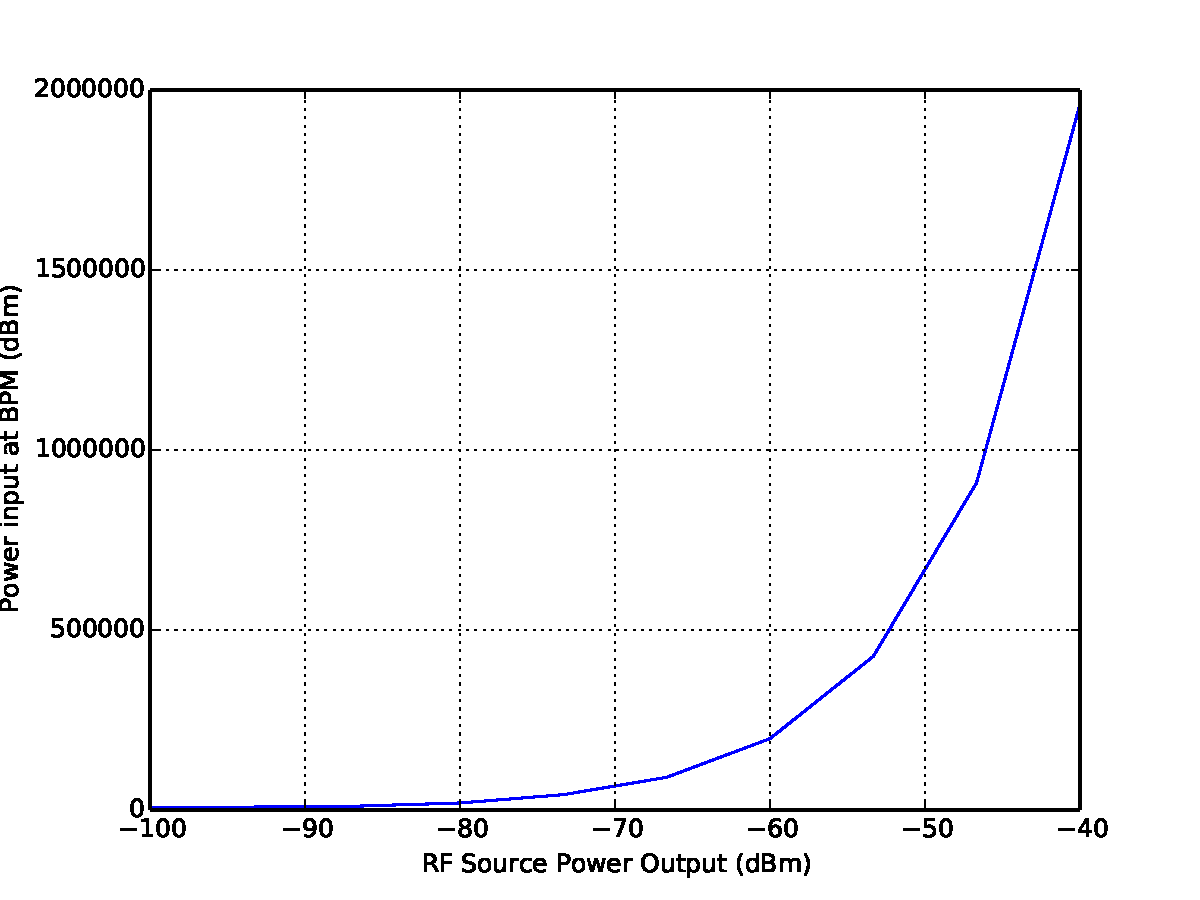
\includegraphics[width=0.8\textwidth]{./Results/power_vs_power.pdf}%
\caption{}%
\end{figure}

%


\begin{figure}[htbp]%
\centering%
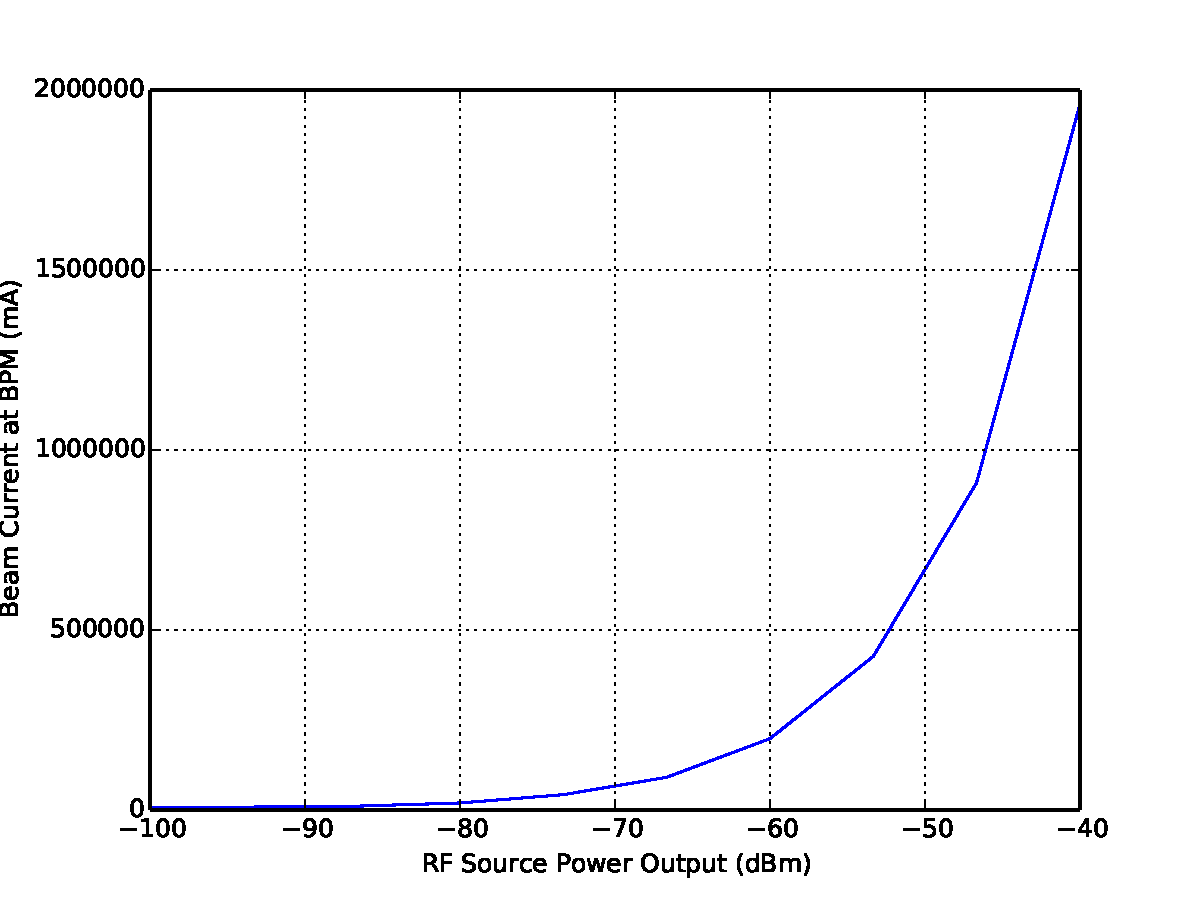
\includegraphics[width=0.8\textwidth]{./Results/power_vs_current.pdf}%
\caption{}%
\end{figure}

%


\begin{figure}[htbp]%
\centering%
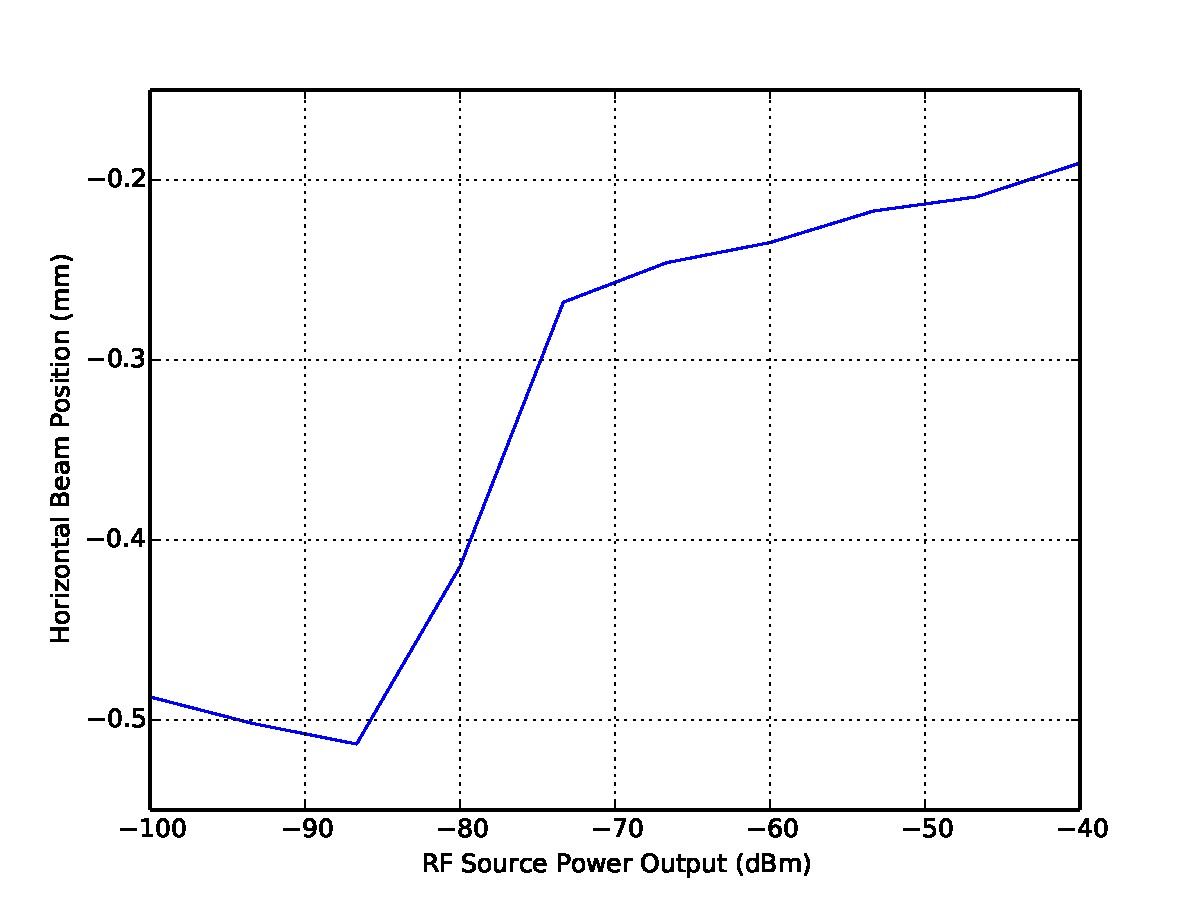
\includegraphics[width=0.8\textwidth]{./Results/power_vs_X.pdf}%
\caption{}%
\end{figure}

%


\begin{figure}[htbp]%
\centering%
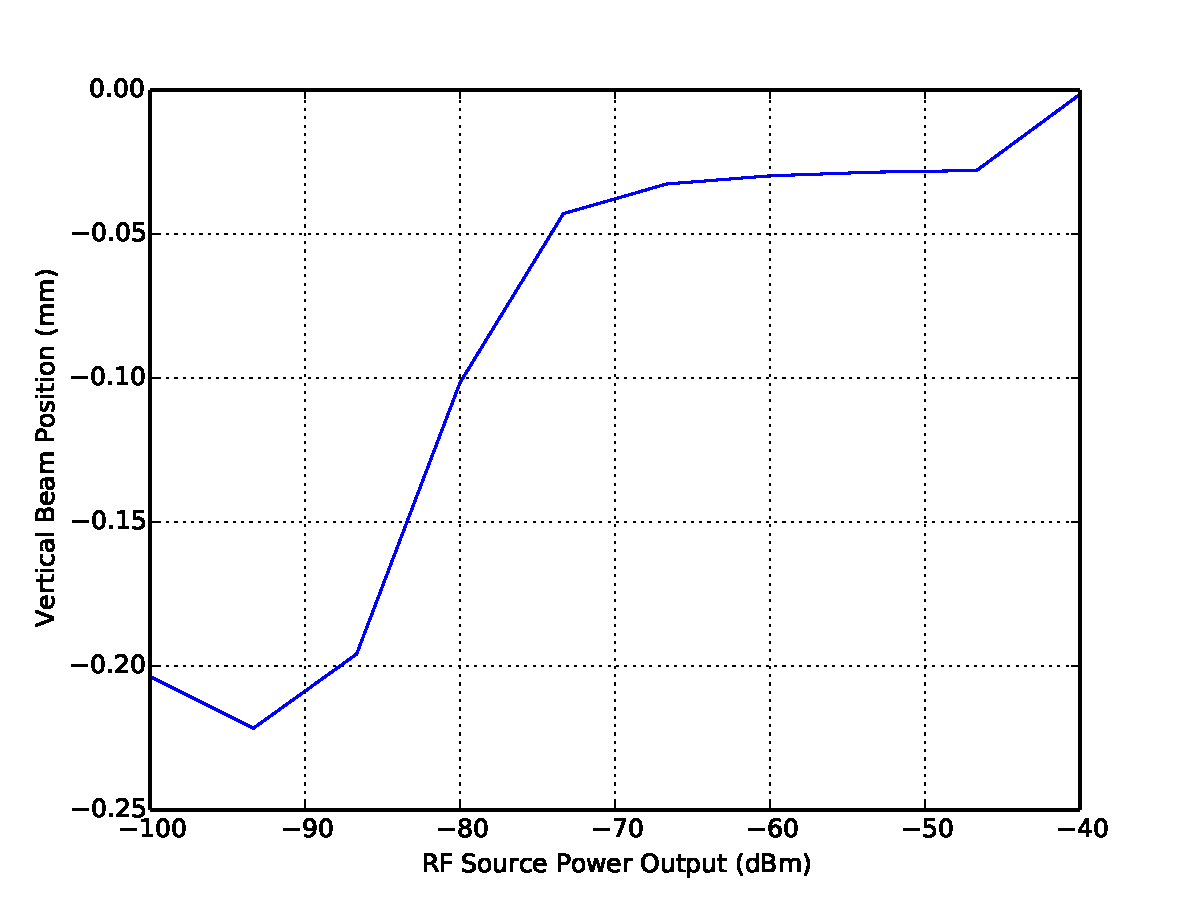
\includegraphics[width=0.8\textwidth]{./Results/power_vs_Y.pdf}%
\caption{}%
\end{figure}

%


\begin{figure}[htbp]%
\centering%
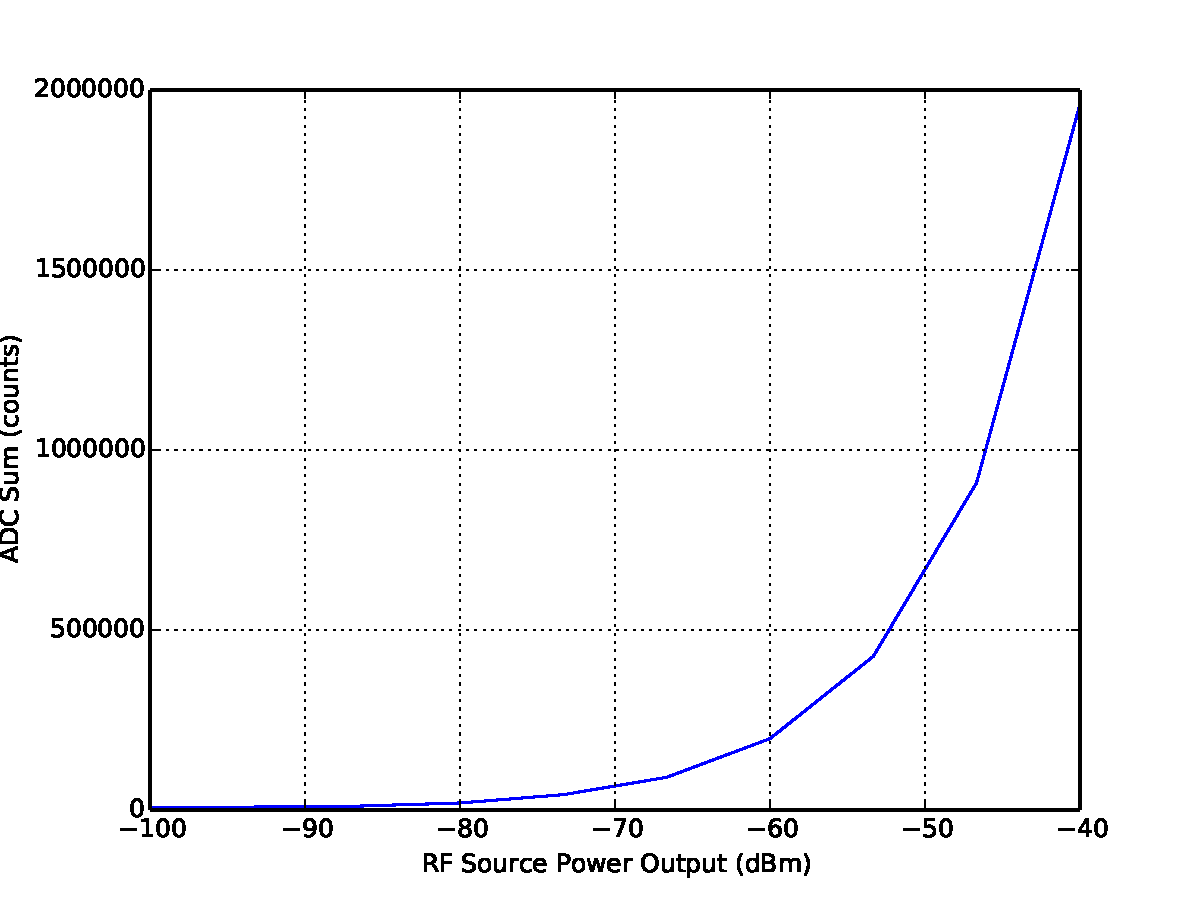
\includegraphics[width=0.8\textwidth]{./Results/power_vs_ADC_sum.pdf}%
\caption{}%
\end{figure}

%
\clearpage%
\section{Fixed amplitude fill pattern test}%
The "Fixed output fill pattern test" is supposed to test the BPM parameters reliance onthe bunch shape that has a variable charge size. The signal suppled by the RF signal generatorwill have a fixed frequency and power output, this is then mixed with a gating signal, modulating the RF signal. The duty cycle of the gating signal is then changed and the BPM parameters recorded. This test will see how these parameters change as the duty cycle is changed.For example, ss the signal provided by the RF is constant the power at the BPM will drop the lower the duty cycle.\\\\%
\textbf{The devices used for this test are:}\\\\%
RF Source Rigol Technologies,DSG3030,DSG3B174500308,00.01.06\\%
Gating Device Rigol Technologies,DSG3030,DSG3B174500308,00.01.06\\%
Libera BPM with the Epics ID "libera:signals:fa" and the MAC Address "00:26:32:46:30:00"\\%
\\%
\textbf{The parameters used in this test are:}\\\\%
Frequency: 499.681 768 20MHz\\%
Output Power: -50.00DBM\\%
Pulse Period: 1.873us\\%
Samples: 30\\

%
\begin{figure}[htbp]%
\centering%
\caption{Changing gate duty cycle, with fixed RF amplitude }%
\begin{tabular}{|c|c|c|c|c|c|}%
\hline%
Duty Cycle&Input Power&BPM Current&X Position&Y Position&ADC Sum\\%
(0{-}1)&(dBm)&(mA)&(mm)&(mm)&(Counts)\\%
\hline%
0.1&83535.4&83535.4&{-}0.15&0.02&83535.4\\%
0.13&111293.92&111293.92&{-}0.14&0.02&111293.92\\%
0.16&139022.98&139022.98&{-}0.14&0.02&139022.98\\%
0.19&162348.2&162348.2&{-}0.14&0.02&162348.2\\%
0.22&190321.7&190321.7&{-}0.14&0.02&190321.7\\%
0.26&218271.81&218271.81&{-}0.14&0.02&218271.81\\%
0.29&246325.8&246325.8&{-}0.14&0.02&246325.8\\%
0.32&274310.26&274310.26&{-}0.14&0.02&274310.26\\%
0.35&297713.96&297713.96&{-}0.14&0.02&297713.96\\%
0.38&325823.48&325823.48&{-}0.14&0.02&325823.48\\%
0.41&353919.4&353919.4&{-}0.14&0.02&353919.4\\%
0.44&382037.4&382037.4&{-}0.14&0.02&382037.4\\%
0.47&410216.98&410216.98&{-}0.14&0.02&410216.98\\%
0.5&433672.22&433672.22&{-}0.14&0.02&433672.22\\%
0.53&461818.84&461818.84&{-}0.14&0.02&461818.84\\%
0.57&490095.88&490095.88&{-}0.14&0.02&490095.88\\%
0.6&518371.36&518371.36&{-}0.14&0.02&518371.36\\%
0.63&546757.31&546757.31&{-}0.14&0.02&546757.31\\%
0.66&574884.12&574884.12&{-}0.14&0.02&574884.12\\%
0.69&598640.15&598640.15&{-}0.14&0.02&598640.15\\%
0.72&626887.61&626887.61&{-}0.14&0.02&626887.61\\%
0.75&655523.62&655523.62&{-}0.14&0.02&655523.62\\%
0.78&683910.04&683910.04&{-}0.14&0.02&683910.04\\%
0.81&712466.52&712466.52&{-}0.14&0.02&712466.52\\%
0.84&736692.63&736692.63&{-}0.14&0.02&736692.63\\%
0.88&765414.23&765414.23&{-}0.14&0.02&765414.23\\%
0.91&794608.84&794608.84&{-}0.14&0.02&794608.84\\%
0.94&824309.95&824309.95&{-}0.14&0.02&824309.95\\%
0.97&855746.31&855746.31&{-}0.14&0.02&855746.31\\%
0.99&879980.53&879980.53&{-}0.14&0.02&879980.53\\%
\hline%
\end{tabular}%
\end{figure}%


\begin{figure}[htbp]%
\centering%
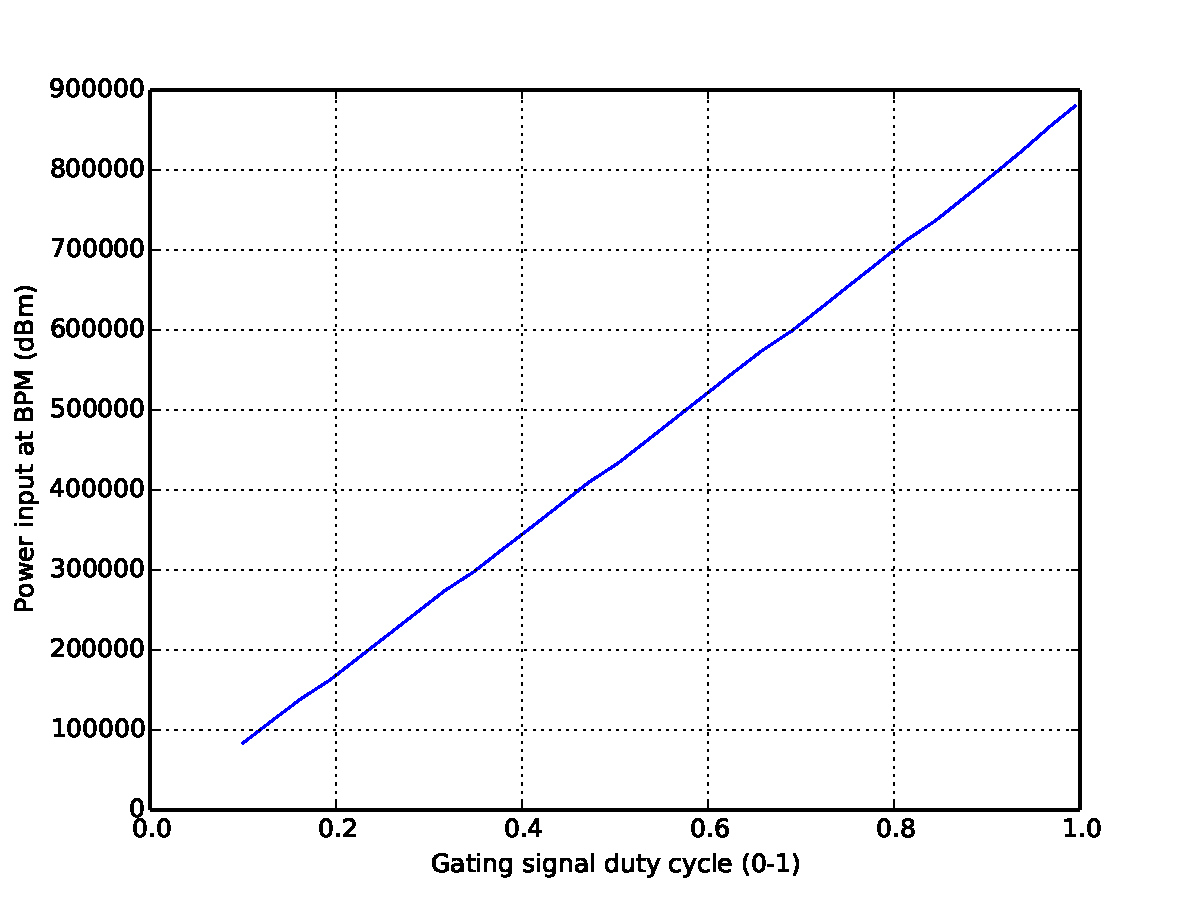
\includegraphics[width=0.8\textwidth]{./Results/DC_vs_power.pdf}%
\caption{}%
\end{figure}

%


\begin{figure}[htbp]%
\centering%
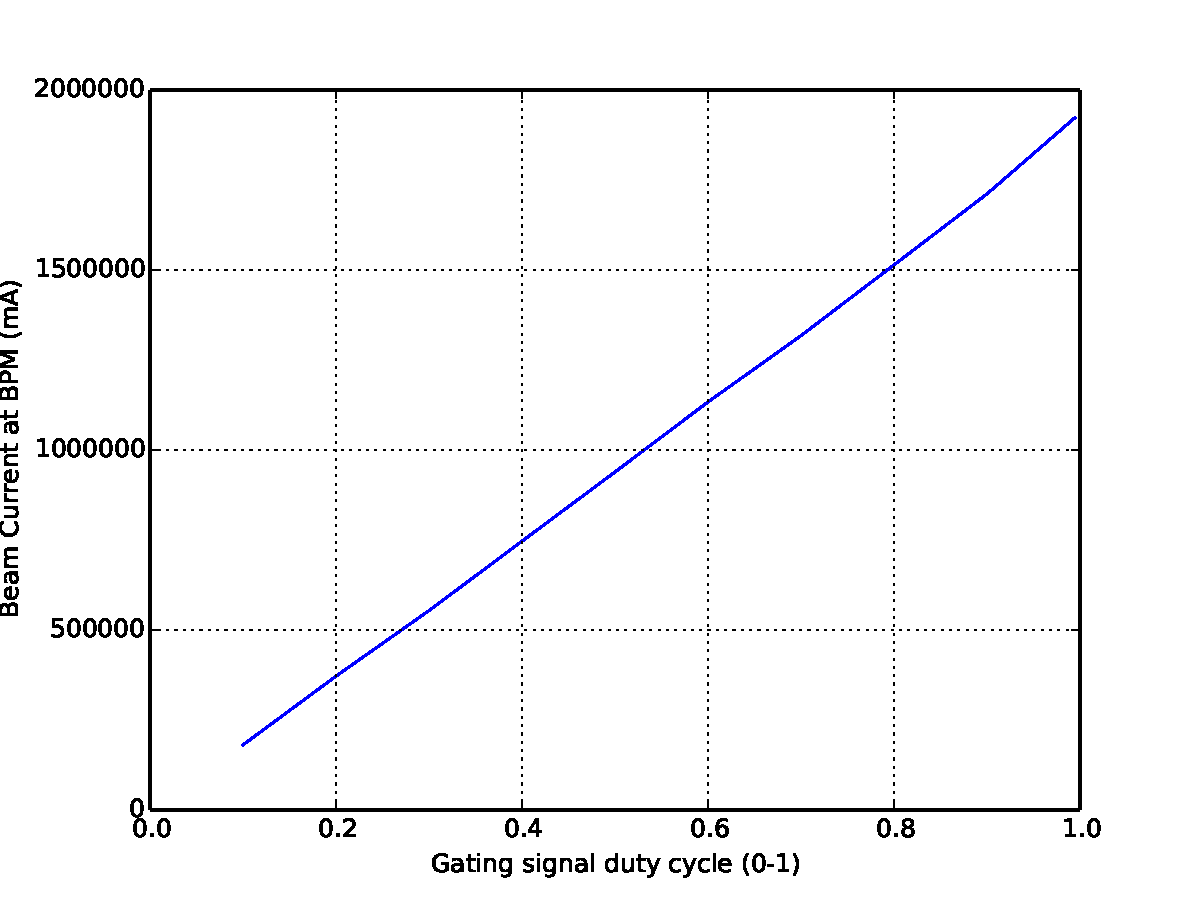
\includegraphics[width=0.8\textwidth]{./Results/DC_vs_current.pdf}%
\caption{}%
\end{figure}

%


\begin{figure}[htbp]%
\centering%
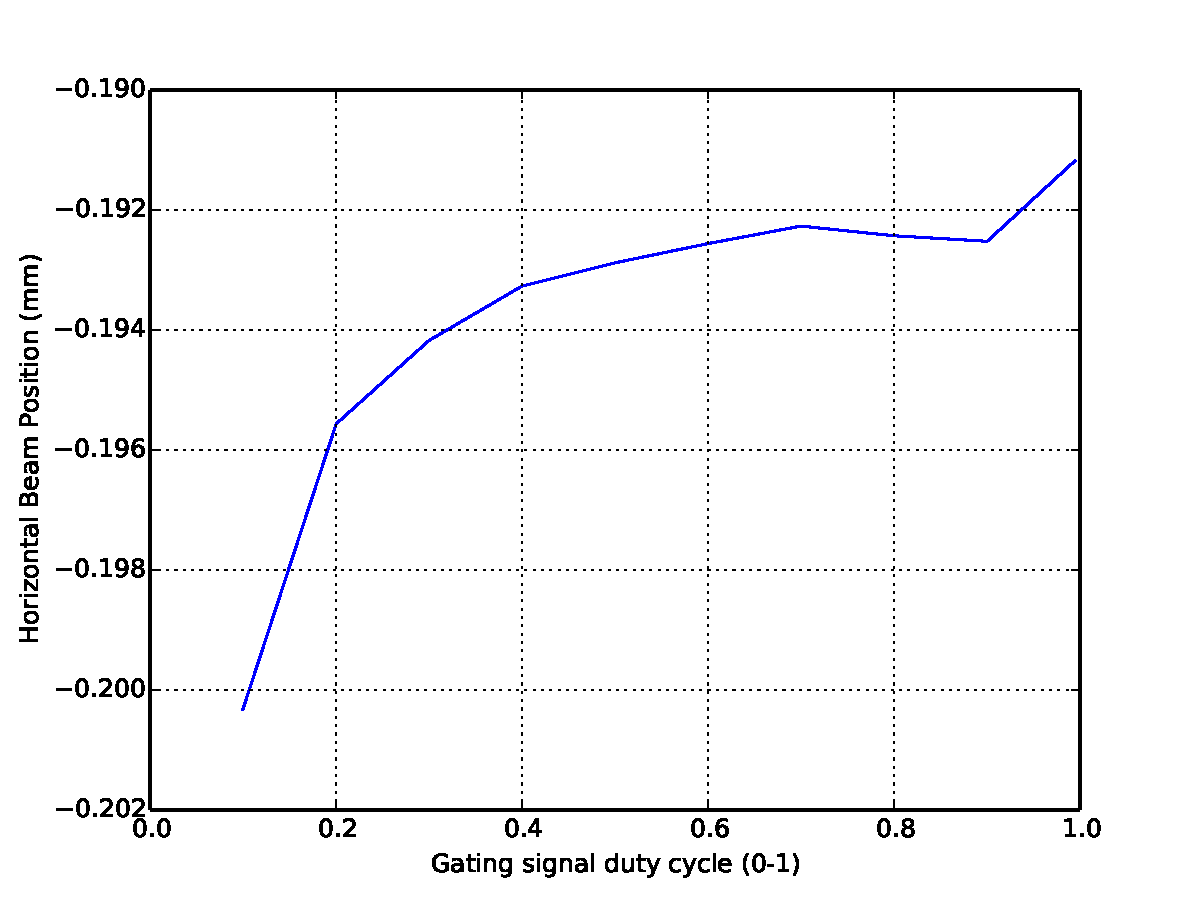
\includegraphics[width=0.8\textwidth]{./Results/DC_vs_X.pdf}%
\caption{}%
\end{figure}

%


\begin{figure}[htbp]%
\centering%
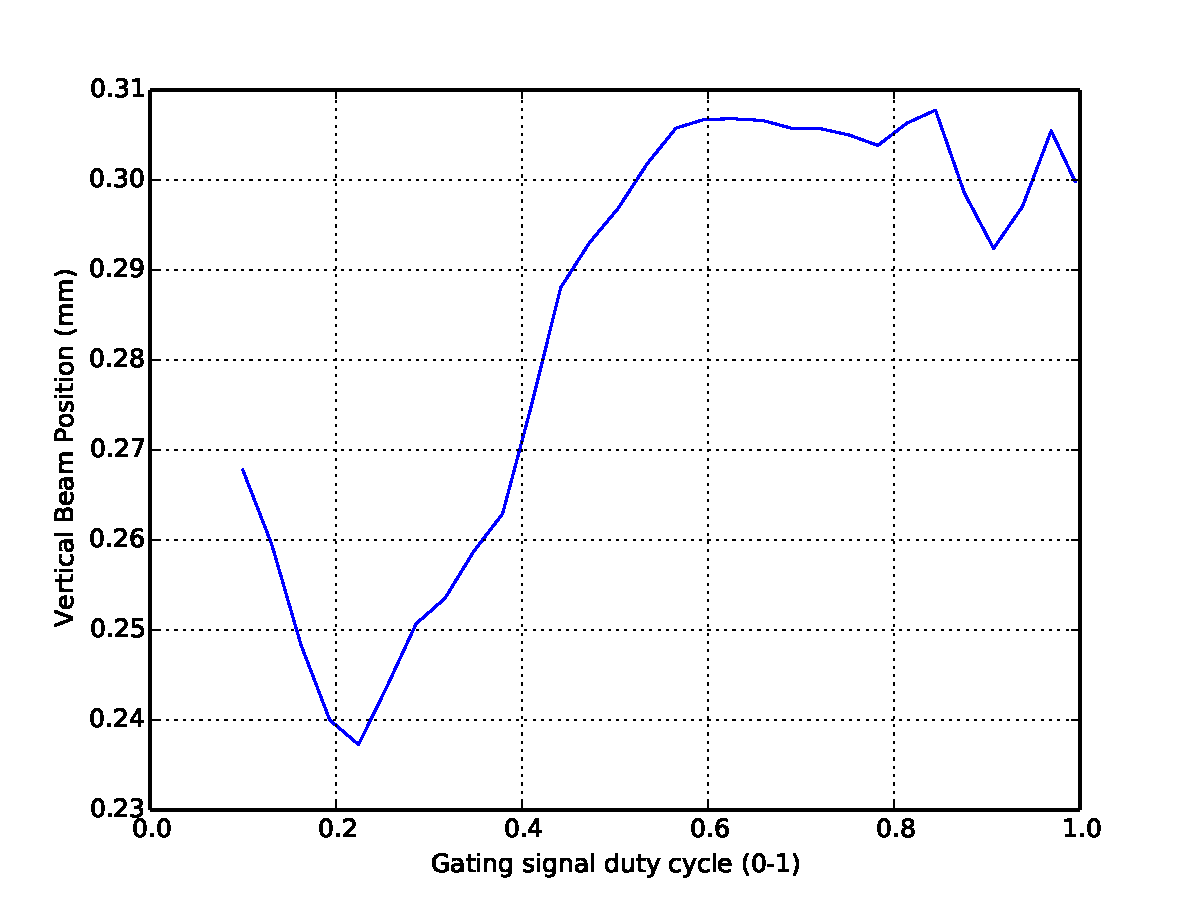
\includegraphics[width=0.8\textwidth]{./Results/DC_vs_Y.pdf}%
\caption{}%
\end{figure}

%


\begin{figure}[htbp]%
\centering%
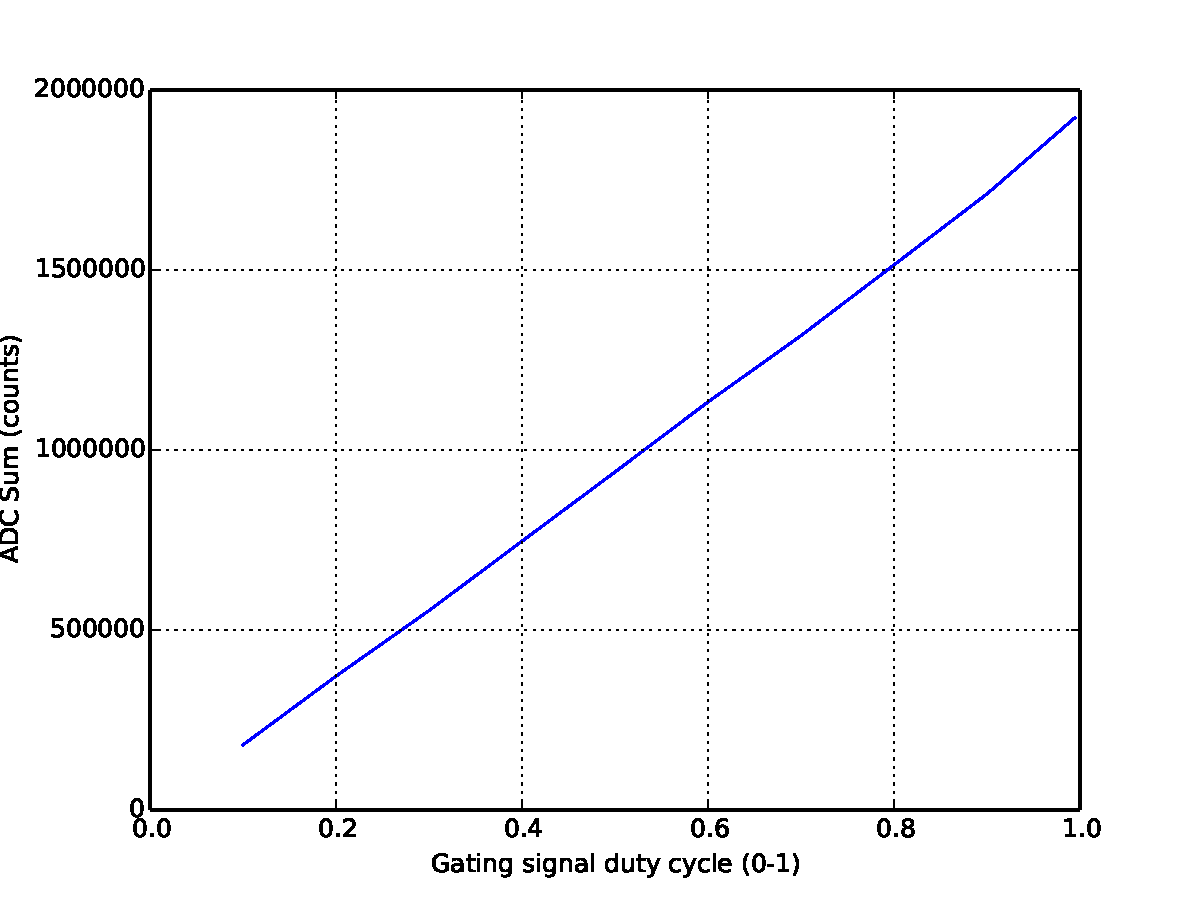
\includegraphics[width=0.8\textwidth]{./Results/DC_vs_ADC_sum.pdf}%
\caption{}%
\end{figure}

%
\clearpage%
\section{Scaled amplitude fill pattern test}%
Scaled output fill pattern test intro text\\\\%
\textbf{The devices used for this test are:}\\\\%
RF Source Rigol Technologies,DSG3030,DSG3B174500308,00.01.06\\%
Gating Device Rigol Technologies,DSG3030,DSG3B174500308,00.01.06\\%
Libera BPM with the Epics ID "libera:signals:fa" and the MAC Address "00:26:32:46:30:00"\\%
\\%
\textbf{The parameters used in this test are:}\\\\%
Frequency: 499.681 768 20MHz\\%
Desired Power: -50\\%
Pulse Period: 1.873us\\%
Samples: 30\\%
Settling time: 3s\\

%
\begin{figure}[htbp]%
\centering%
\caption{Changing gate duty cycle, with fixed RF amplitude }%
\begin{tabular}{|c|c|c|c|c|c|c|}%
\hline%
Duty Cycle&Output Power&Input Power&BPM Current&X Position&Y Position&ADC Sum\\%
(0{-}1)&(dBm)&(dBm)&(mA)&(mm)&(mm)&(Counts)\\%
\hline%
0.1&{-}40.0&269973.94&269973.94&{-}0.12&0.05&269973.94\\%
0.13&{-}40.0&359435.14&359435.14&{-}0.12&0.05&359435.14\\%
0.16&{-}40.0&449798.28&449798.28&{-}0.12&0.05&449798.28\\%
0.19&{-}40.0&523724.52&523724.52&{-}0.12&0.05&523724.52\\%
0.22&{-}40.0&615447.32&615447.32&{-}0.12&0.05&615447.32\\%
0.26&{-}40.0&706212.52&706212.52&{-}0.12&0.05&706212.52\\%
0.29&{-}40.0&796933.98&796933.98&{-}0.12&0.05&796933.98\\%
0.32&{-}40.02&882587.6&882587.6&{-}0.12&0.05&882587.6\\%
0.35&{-}40.83&870120.01&870120.01&{-}0.12&0.05&870120.01\\%
0.38&{-}41.57&875173.02&875173.02&{-}0.12&0.05&875173.02\\%
0.41&{-}42.27&873861.6&873861.6&{-}0.12&0.05&873861.6\\%
0.44&{-}42.9&831926.22&831926.22&{-}0.12&0.05&831926.22\\%
0.47&{-}43.49&830293.86&830293.86&{-}0.13&0.04&830293.86\\%
0.5&{-}44.04&823727.9&823727.9&{-}0.13&0.04&823727.9\\%
0.53&{-}44.56&821939.17&821939.17&{-}0.13&0.04&821939.17\\%
0.57&{-}45.05&824357.36&824357.36&{-}0.13&0.04&824357.36\\%
0.6&{-}45.51&828802.22&828802.22&{-}0.13&0.04&828802.22\\%
0.63&{-}45.95&827175.52&827175.52&{-}0.13&0.03&827175.52\\%
0.66&{-}46.38&907083.67&907083.67&{-}0.13&0.04&907083.67\\%
0.69&{-}46.77&889307.44&889307.44&{-}0.13&0.03&889307.44\\%
0.72&{-}47.16&888339.9&888339.9&{-}0.13&0.03&888339.9\\%
0.75&{-}47.52&891307.6&891307.6&{-}0.13&0.03&891307.6\\%
0.78&{-}47.87&888684.07&888684.07&{-}0.13&0.03&888684.07\\%
0.81&{-}48.21&894887.37&894887.37&{-}0.14&0.03&894887.37\\%
0.84&{-}48.53&884800.66&884800.66&{-}0.14&0.03&884800.66\\%
0.88&{-}48.85&886991.17&886991.17&{-}0.14&0.03&886991.17\\%
0.91&{-}49.15&889890.4&889890.4&{-}0.14&0.02&889890.4\\%
0.94&{-}49.44&889808.02&889808.02&{-}0.14&0.02&889808.02\\%
0.97&{-}49.73&894195.05&894195.05&{-}0.14&0.02&894195.05\\%
0.99&{-}49.95&901190.15&901190.15&{-}0.14&0.02&901190.15\\%
\hline%
\end{tabular}%
\end{figure}%


\begin{figure}[htbp]%
\centering%
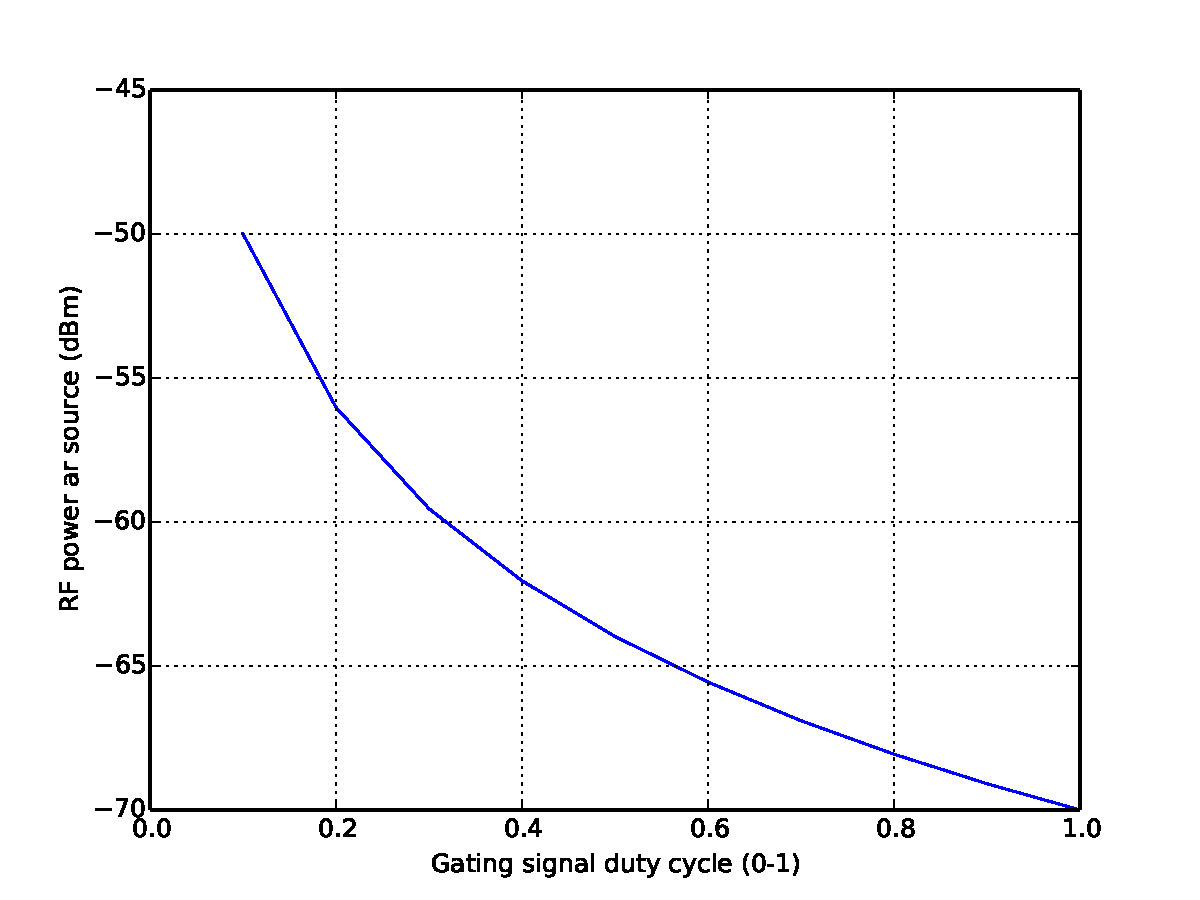
\includegraphics[width=0.8\textwidth]{./Results/scaled_DC_vs_Out_power.pdf}%
\caption{}%
\end{figure}

%


\begin{figure}[htbp]%
\centering%
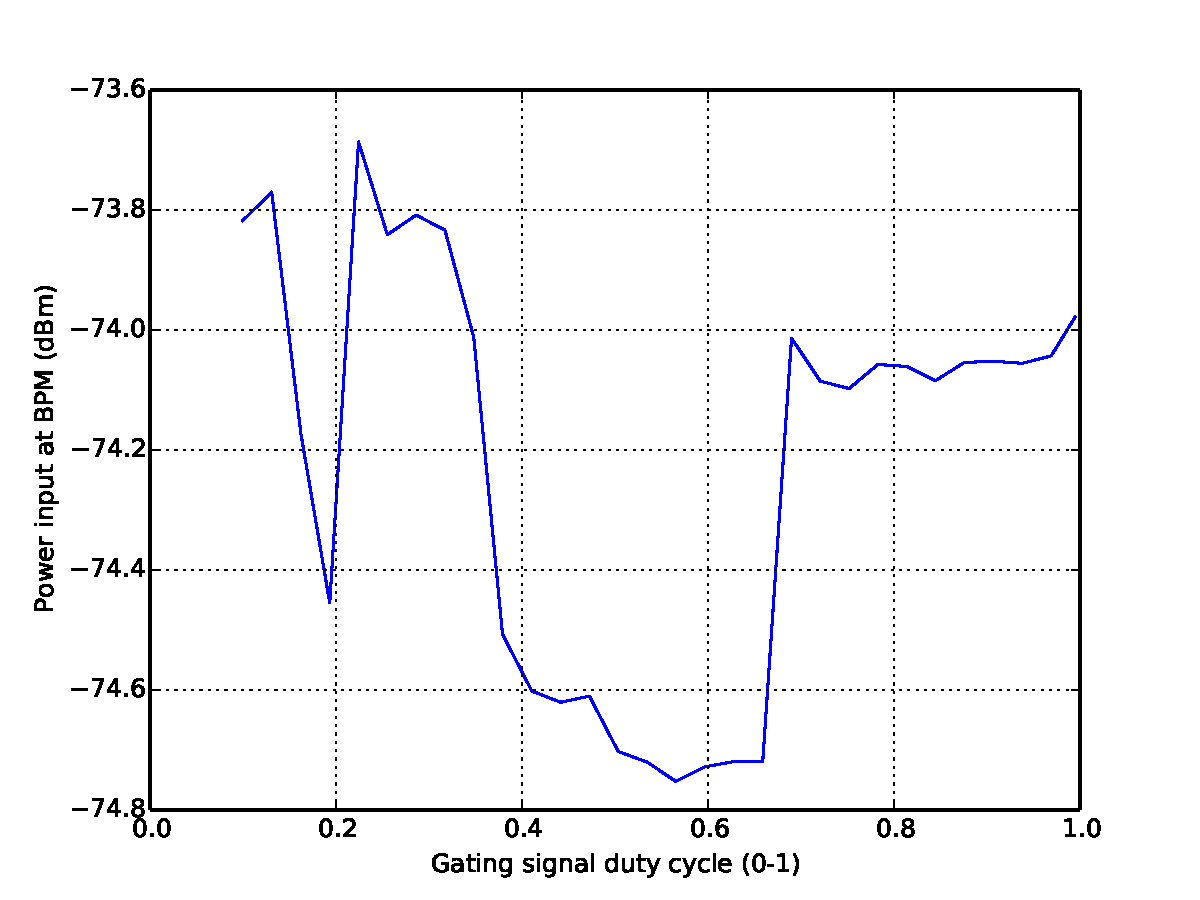
\includegraphics[width=0.8\textwidth]{./Results/scaled_DC_vs_In_power.pdf}%
\caption{}%
\end{figure}

%


\begin{figure}[htbp]%
\centering%
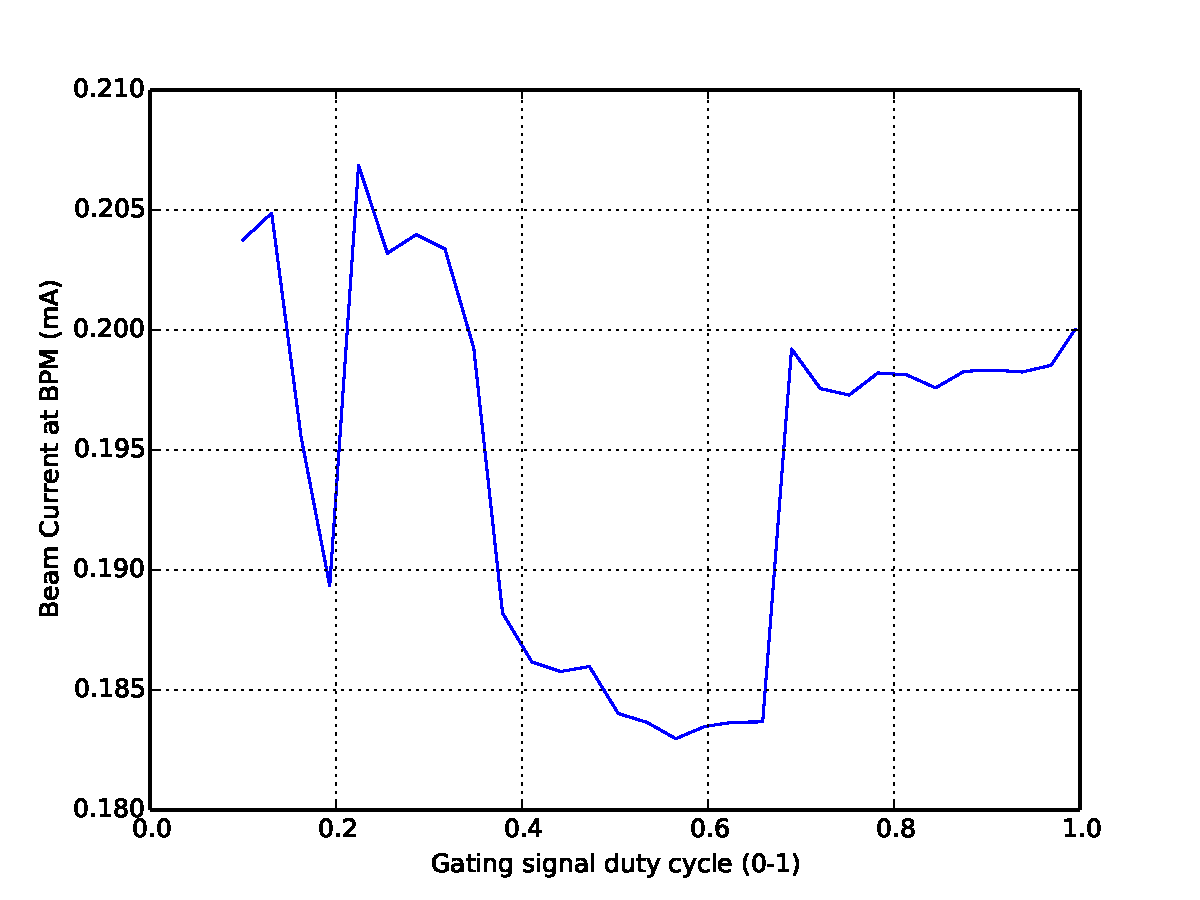
\includegraphics[width=0.8\textwidth]{./Results/scaled_DC_vs_current.pdf}%
\caption{}%
\end{figure}

%


\begin{figure}[htbp]%
\centering%
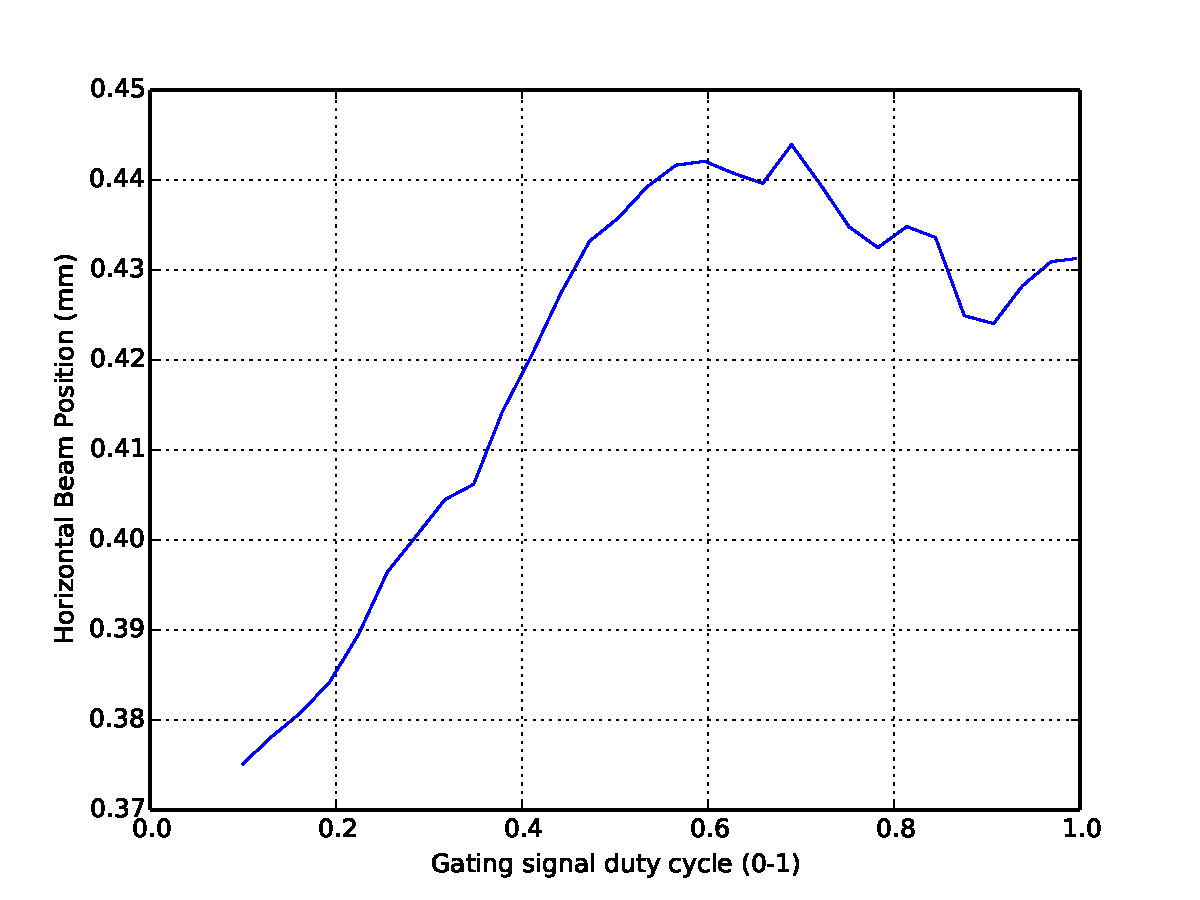
\includegraphics[width=0.8\textwidth]{./Results/scaled_DC_vs_X.pdf}%
\caption{}%
\end{figure}

%


\begin{figure}[htbp]%
\centering%
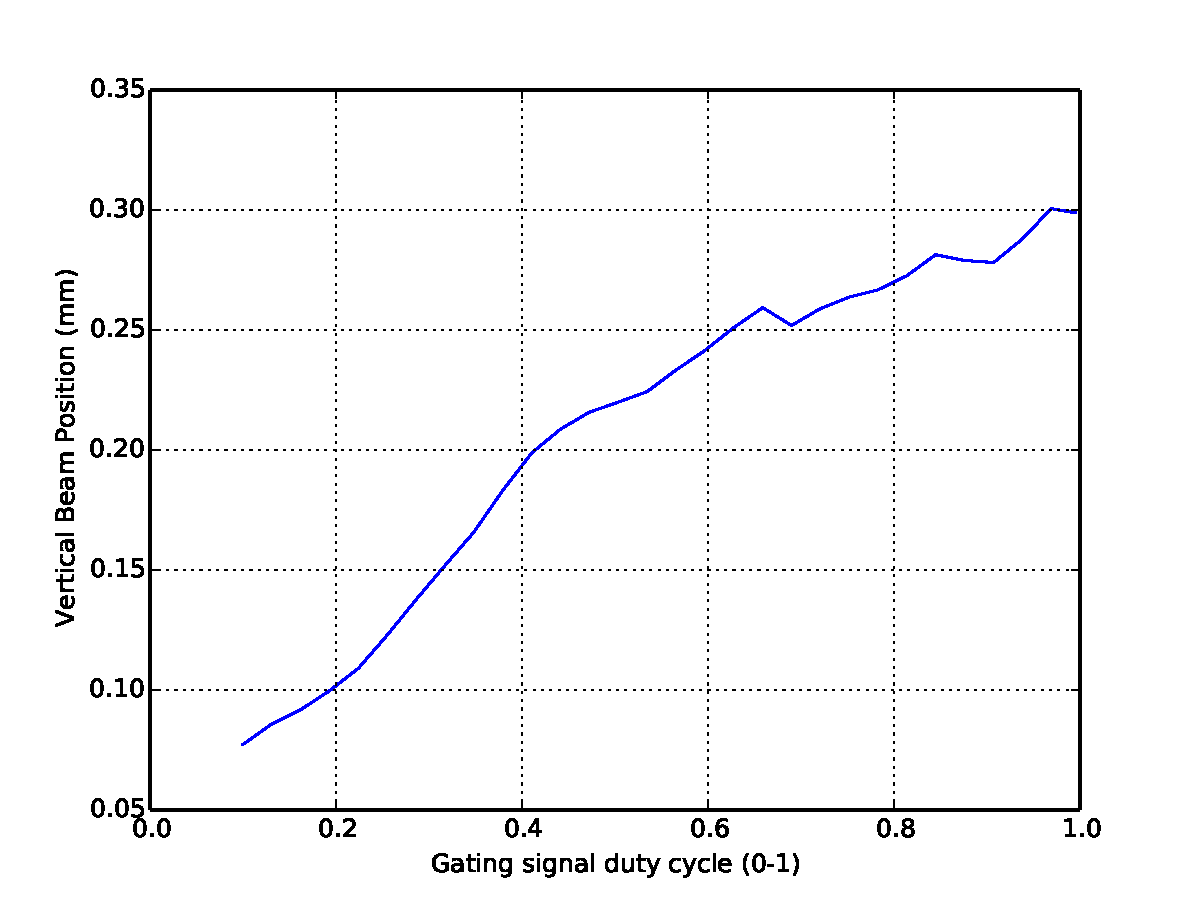
\includegraphics[width=0.8\textwidth]{./Results/scaled_DC_vs_Y.pdf}%
\caption{}%
\end{figure}

%


\begin{figure}[htbp]%
\centering%
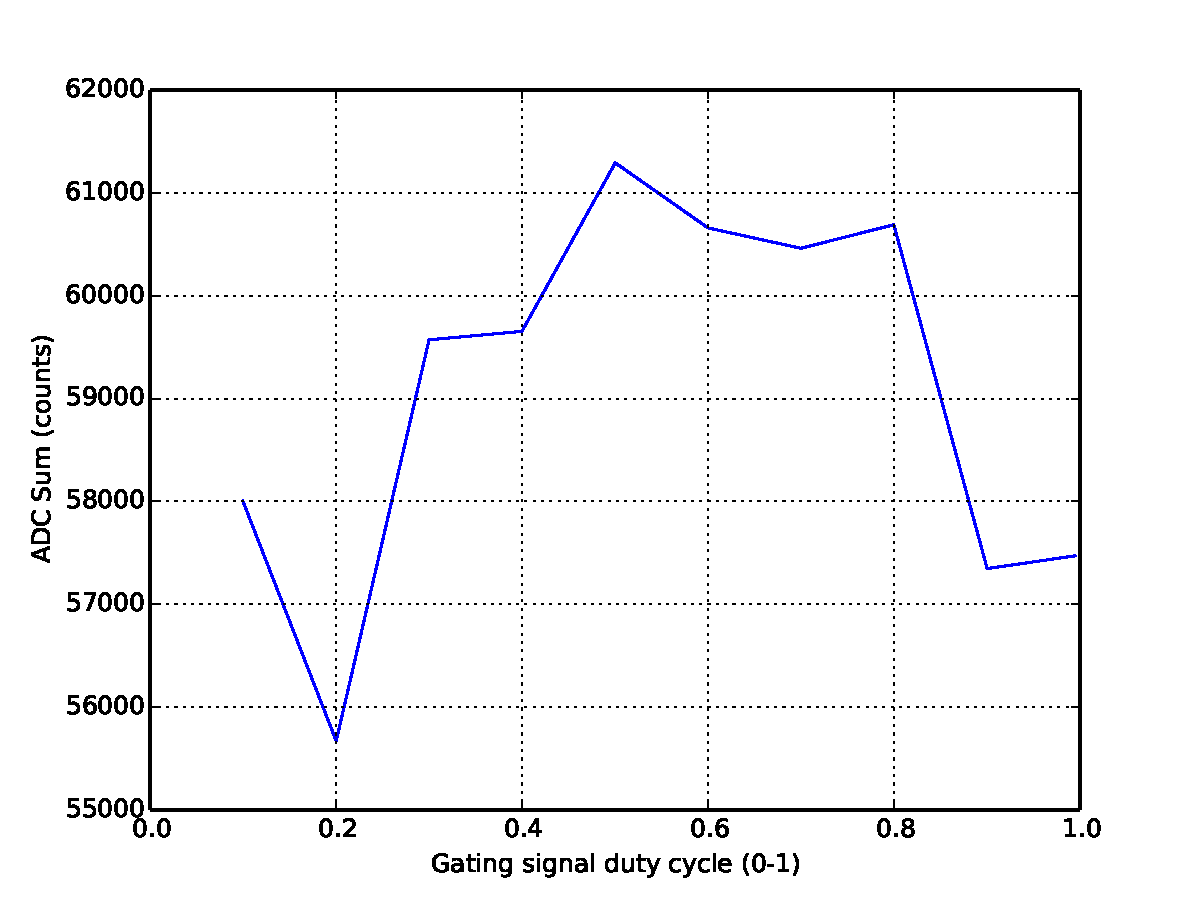
\includegraphics[width=0.8\textwidth]{./Results/scaled_DC_vs_ADC_Sum.pdf}%
\caption{}%
\end{figure}

%
\end{document}